\documentclass[aps,pra,reprint,amsmath,amssymb,floatfix,nofootinbib]{revtex4-2}

\usepackage{graphicx}
\usepackage{bm}

\begin{document}

\title{Wigner Resolution from the Action Capacity of the State}

\author{Brian S. Mulloy}
\email{bmulloy@umich.edu}

\date{\today}

\begin{abstract}

\end{abstract}

\maketitle

\begin{figure*}[t]
\includegraphics[width=\textwidth]{figures/}
\caption{Squeezed vacuum ($r=0.5$), harmonic oscillator $n=1$, Morse $n=8$,
and double-well $n=5$.}
\label{fig:eigen}
\end{figure*}


\begin{figure*}[t]
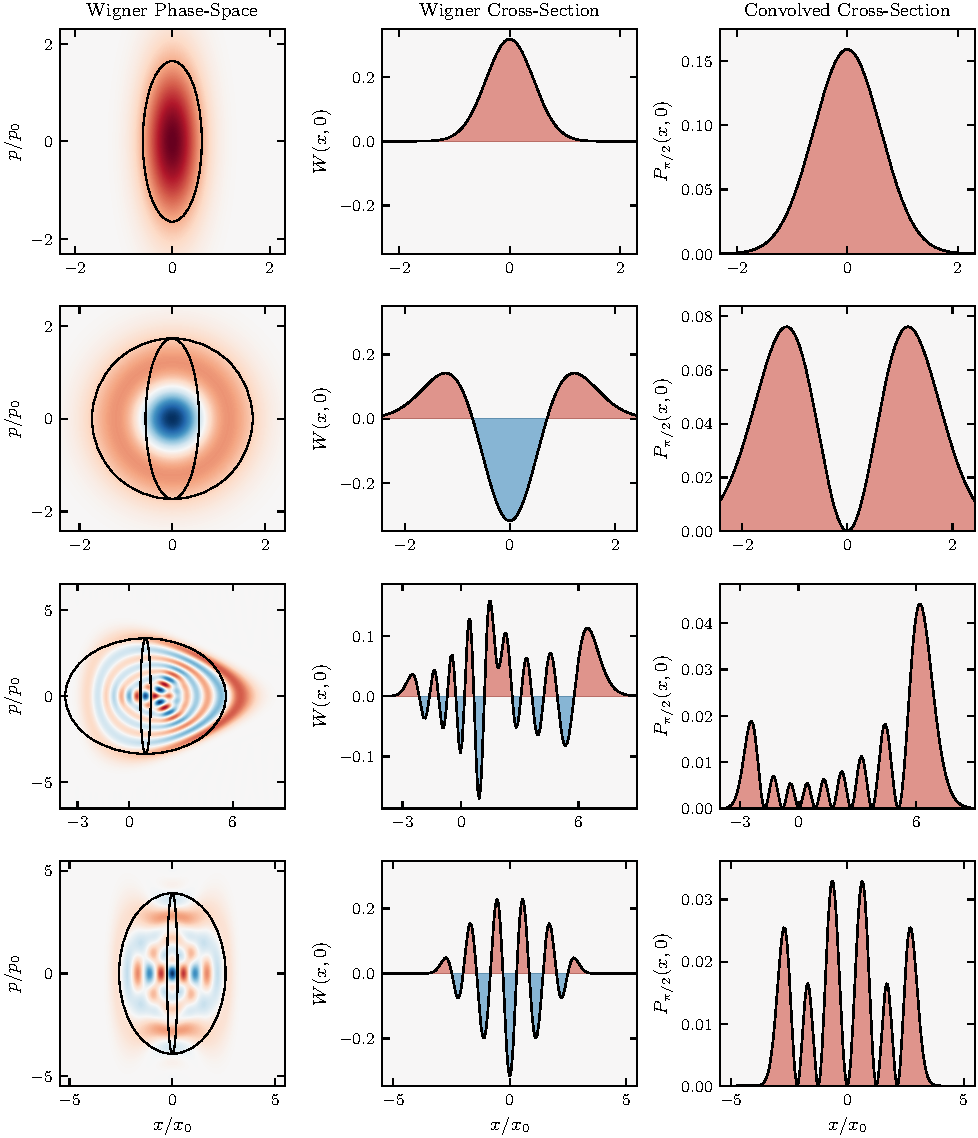
\includegraphics[width=\textwidth]{figures/eigen}
\caption{Squeezed vacuum ($r=0.5$), harmonic oscillator $n=1$, Morse $n=8$,
and double-well $n=5$.}
\label{fig:eigen}
\end{figure*}

%\bibliography{main}

\end{document}